\newcommand{\halfangle}{10}
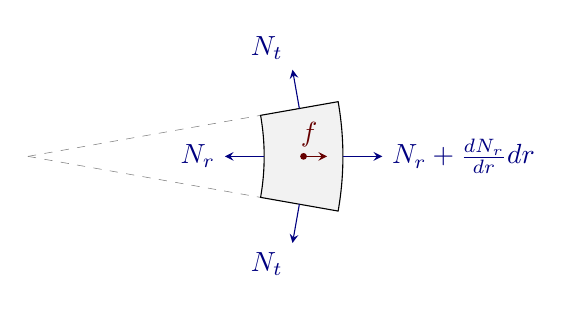
\begin{tikzpicture}[scale=2]
	%The bisected dotted lines
	\begin{scope}[dashed,gray,very thin]
		\draw (0,0) -- (\halfangle:1.5 cm);
		\draw (0,0) -- (-\halfangle:1.5 cm);
	\end{scope}
	%Draw the area element
	\filldraw[fill=gray!10,draw=black] (-\halfangle:1.5 cm)  arc(-\halfangle:\halfangle:1.5 cm) -- (\halfangle:2 cm) arc(\halfangle:-\halfangle:2 cm) -- cycle;
	%Draw the force lines and labels
	\begin{scope}[->, blue!50!black,>=stealth]
		\draw (0:2 cm) -- +(0:.25 cm) node[anchor=west]{$N_r+\frac{dN_r}{dr} dr$};
		\draw (0:1.5 cm) -- +(0:-.25 cm) node[anchor=east]{$N_r$};
		\draw (\halfangle:1.75 cm) -- +(90+\halfangle:.25 cm) node[anchor=south east]{$N_t$};
		\draw (-\halfangle:1.75 cm) -- +(-90-\halfangle:.25 cm) node[anchor=north east]{$N_t$};
		\filldraw[red!40!black] (1.75,0) circle(.5pt);
		\draw[red!40!black] (1.75,0) -- +(.15,0) node[anchor=south east]{$f$};
	\end{scope}
\end{tikzpicture}